\documentclass[a4paper,12pt]{article}

%%% Работа с русским языком
\usepackage{cmap}					% поиск в PDF
\usepackage{mathtext} 				% русские буквы в формулах
\usepackage[T2A]{fontenc}			% кодировка
\usepackage[utf8]{inputenc}			% кодировка исходного текста
\usepackage[english,russian]{babel}	% локализация и переносы
\usepackage{comment}


%%% Дополнительная работа с математикой
\usepackage{amsfonts,amssymb,amsthm,mathtools} % AMS
\usepackage{amsmath}
\usepackage{icomma} % "Умная" запятая: $0,2$ --- число, $0, 2$ --- перечисление

%% Номера формул
%\mathtoolsset{showonlyrefs=true} % Показывать номера только у тех формул, на которые есть \eqref{} в тексте.

%% Шрифты
\usepackage{euscript}	 % Шрифт Евклид
\usepackage{mathrsfs} % Красивый матшрифт

\usepackage{extsizes} % Возможность сделать 14-й шрифт
\usepackage{geometry} % Простой способ задавать поля
\geometry{top=25mm}
\geometry{bottom=35mm}
\geometry{left=20mm}
\geometry{right=20mm}

\usepackage{chngcntr}
\usepackage{hyperref}

\usepackage{setspace} % Интерлиньяж
%\onehalfspacing % Интерлиньяж 1.5
%\doublespacing % Интерлиньяж 2
%\singlespacing % Интерлиньяж 1

\usepackage{lastpage} % Узнать, сколько всего страниц в документе.
\usepackage{soulutf8} % Модификаторы начертания

\counterwithin*{equation}{section}
\counterwithin*{equation}{subsection}



%% Свои команды
\DeclareMathOperator{\sgn}{\mathop{sgn}}

%% Перенос знаков в формулах (по Львовскому)
\newcommand*{\hm}[1]{#1\nobreak\discretionary{}
{\hbox{$\mathsurround=0pt #1$}}{}}

%%% Работа с картинками
\usepackage{graphicx}  % Для вставки рисунков
\graphicspath{{images/}{images2/}}  % папки с картинками
\setlength\fboxsep{3pt} % Отступ рамки \fbox{} от рисунка
\setlength\fboxrule{1pt} % Толщина линий рамки \fbox{}
\usepackage{wrapfig} % Обтекание рисунков и таблиц текстом

%%% Работа с таблицами
\usepackage{array,tabularx,tabulary,booktabs} % Дополнительная работа с таблицами
\usepackage{longtable}  % Длинные таблицы
\usepackage{multirow} % Слияние строк в таблице
\usepackage{graphicx}
\usepackage{fancyhdr}
\usepackage{hyperref}
\usepackage{booktabs}

\newcommand{\lt}{\left}
\newcommand{\rt}{\right}
\newcommand{\al}{\alpha}

\pagestyle{fancy}
\fancyhf{}
\pagestyle{plain} % нумерация вкл.

\rhead{\today}
\lhead{Соколов Игорь, группа 573}

%%% Заголовок
\author{Соколов Игорь, группа 573}
\title{ДЗ 3 по Методам Оптимизации. \newline Отделимость. Проекция. Опорная гиперплоскость}
\date{\today}

\begin{document} % конец преамбулы, начало документа

\maketitle



\section{}

Найти $\pi_S (y) = \pi$, если $S = \{x \in \mathbb{R}^n \mid c^T x \ge b \}$

\vspace{\baselineskip}

\textbf{Решение:}

\vspace{\baselineskip}

Рассмотрим два случая:

1. $y \in S$:

Тогда $\pi(y) = y$.

\vspace{\baselineskip}

2. $y \notin S$

Заметим, что $\{x \in \mathbb{R}^n \mid c^T x \ge b \}$ задает полупространство, тогда $S$ - выпуклое замкнутое множество.

$\Rightarrow$ $\pi_S(y) \in \partial S = \{x \in \mathbb{R}^n \mid c^T x = b \}$

\vspace{\baselineskip}

Строим гипотезу: 

$\pi = y + \alpha c$. Коэффициент $\alpha$ подбирается так, чтобы $\pi \in S$: $c^T \pi = b$, т.е.: $$c^T (y + \alpha c) = b$$
 $$c^Ty + \alpha c^T c = b$$
 $$c^Ty = b - \alpha c^T c$$
 
 $$\alpha = \frac{b - c^Ty}{c^Tc}$$
 
Проверяем неравенство для выпуклого замкнутого множества: $(\pi - y)^T(x - \pi) \ge 0$


 $$(y + \alpha c - y)^T(x - y - \alpha c) = $$
 $$ \alpha c^T(x - y - \alpha c) = $$
 $$ \alpha (c^Tx) - \alpha (c^T y) - \alpha^2 c^Tc) = $$
 $$ \alpha b - \alpha (b - \alpha c^T c) - \alpha^2 c^Tc = $$
 $$ \alpha b - \alpha b + \alpha^2 c^T c - \alpha^2 c^Tc = 0 \ge 0$$


\textbf{Ответ:} $\pi = y + \dfrac{b - c^Ty}{c^Tc}c$

\section{}

Найти $\pi_S (y) = \pi$, если $S = \{x \in \mathbb{R}^n \mid x = x_0 + X\alpha, X \in \mathbb{R}^{n \times m},  \alpha \in \mathbb{R}^{m}\}$, $y \notin S$

\vspace{\baselineskip}

\textbf{Решение:}

\vspace{\baselineskip}

Пусть $S = x_0 + S'$

Тогда $S' = \{x' \in \mathbb{R}^n \mid x' = X\alpha, X \in \mathbb{R}^{n \times m},  \alpha \in \mathbb{R}^{m}\}$

\begin{equation}\label{eq_pi}
\Rightarrow \pi_S (y) = x_0+\pi_{S'} (y)
\end{equation}

Тогда сведем задачу к нахождению $\pi_{S'} (y) = \pi'$

$$x' = X\alpha$$
$$X^Tx' = (X^TX)\alpha$$
$$(X^TX)^{-1}X^Tx' = \alpha$$

где $(X^TX)$ - квадратная матрица.

Пусть $A = (X^TX)^{-1}X^T$.

Тогда $$Ax' = \alpha$$

$\Rightarrow$
\begin{equation}\label{eq_S'}
S' = \{x' \in \mathbb{R}^n \mid Ax' = \alpha, X \in \mathbb{R}^{n \times m},  \alpha \in \mathbb{R}^{m}\}
\end{equation}

Имеем систему линейных уравнений относительно $x'$.

Геометрически это можно интерпретировать как перечение $n$ гиперплоскостей в $\mathbb{R}^{m}$.

\vspace{\baselineskip}

Рассмотрим расширенную матрицу системы $\lt(A|\al\rt)$:

\vspace{\baselineskip}

1. Если $n > m$ или $n < m$:

1.1. Если есть повторяющиеся строки в $\lt(A|\al\rt)$,то уберем их - множество решений не изменится.

1.2. Если есть две повторяющиеся строки в $A$ при этом они отличаются в правой частью, то это соответствует двум параллельным гиперплоскостям. В таком случае система не будет иметь решение и  $S'=\varnothing$

$\Rightarrow \nexists \pi_{S'}(y)$ (не существует проекции на пустое множество)

\vspace{\baselineskip}

2. Если $n = m$:

2.1 $det(A) = 0$:

По правилу Крамера решений либо не существует(параллельные гиперплоскости), либо бесконечно много(совпадающие гиперплоскости).

2.2 $det(A) \neq 0$:

По правилу Крамера решение существует и единственно.

\vspace{\baselineskip}

Строим гипотезу: $\pi_{S'}(y) = y + \sum\limits_{i=1}^n\beta_i A_i = y + A^T \beta$.

Столбцы матрицы $A^T$ есть нормальные вектора гиперплоскостей.

Коэффициент $\beta$ подбирается так, чтобы $\pi' \in S'$: $A \pi' = \al$, т.е.: 
$$A(y + A^T\beta) = \alpha$$

\begin{equation}\label{eq_beta}
Ay = \alpha - A A^T\beta
\end{equation}

Проверяем неравенство для выпуклого замкнутого множества: $(\pi - y)^T(x' - \pi) \ge 0$
$$(y + A^T\beta  - y)^T(x' - y - A^T\beta) = $$
$$ \beta^T A(x' - y - A^T\beta) = $$
$$ \beta^T (Ax') - \beta^T (A y) - \beta^T AA^T \beta) = $$
$$ \beta^T \alpha - \beta^T (\alpha - A A^T\beta) - \beta^T AA^T \beta = $$
$$ \beta^T \alpha - \beta^T \alpha + \beta^T AA^T \beta - \beta^T AA^T \beta = 0 \ge 0$$

$\Rightarrow$ выполнено.

\vspace{\baselineskip}

Из уравнения \ref{eq_beta} находим 

$\beta = (AA^T)^{-1}(\al - Ay)$

$\Rightarrow \pi_{S'}(y) = y + A^T(AA^T)^{-1}(\al - Ay) $

\vspace{\baselineskip}

В силу \ref{eq_pi} имеем 

\begin{equation}\label{eq_pi2}
\pi_{S}(y) = x_0 + y + A^T(AA^T)^{-1}(\al - Ay)
\end{equation}

\vspace{\baselineskip}

$$A = (X^TX)^{-1}X^T$$
$$A^T = \lt((X^TX)^{-1}X^T\rt)^T = X((X^TX)^{-1})^T = X((X^TX)^T)^{-1} = X(X^TX)^{-1}  $$
$$\lt(AA^T\rt)^{-1} = \lt((X^TX)^{-1}X^TX(X^TX)^{-1}\rt)^{-1} = \lt((X^TX)^{-1}\rt)^{-1} = X^TX  $$
$$A^T(AA^T)^{-1} = X(X^TX)^{-1}(X^TX) = X$$

И тогда \ref{eq_pi2} переписывается как

$$\pi_{S}(y) = x_0 + y + X\lt(\al - (X^TX)^{-1}X^Ty\rt)$$
$$\pi_{S}(y) = x_0 + y + X\al - X(X^TX)^{-1}X^Ty$$
$$\pi_{S}(y) = x_0 + X\al + (\mathbb{E} - X(X^TX)^{-1}X^T)y$$

\textbf{Ответ:} $\pi_{S}(y) = x_0 + X\al + (\mathbb{E} - X(X^TX)^{-1}X^T)y$

%3

\section{}

Построить гиперплоскость, разделяющую $S_1$ и $S_2$:
$$S_1 = \left\{ x \in \mathbb{R}^n \mid x_1^2 + x_2^2 + \ldots + x_n^2 \le 1\right\}, \;\;\; S_2 = \left\{ x \in \mathbb{R}^n \mid x_1^2 + x_2^2 + \ldots + x_{n-1}^2 + 1 \le x_n \right\}$$

\vspace{\baselineskip}

\textbf{Решение:}

\vspace{\baselineskip}

Найдем $\mathbf{\partial S_1 \cap \partial S_2}$

$\begin{cases}
\sum\limits_{i=1}^n x_i^2 = 1  \\
\sum\limits_{i=1}^{n-1} (x_i^2) +1= x_n 
\end{cases}$

\vspace{\baselineskip}

Вычтем второе уравнение из первого\\
$\Longrightarrow$  $$x_n^2 -1 = 1 - x_n$$
$$x_n^2 + x_n -2 = 0$$
$$x_{n_{1,2}} = -2; 1$$

Из двух корней подходит только $x_n = 1$, так как в левой части второго уравнения cистемы стоит положительное число.

$\Rightarrow$
$$ x_1= x_2  = \ldots = x_{n-1} = 0 $$

т.е. множества пересекаются в точке $x_0 = (0, 0, \ldots, 0, 1)$

Построим касательные плоскости к обеим поверхностям в точке пересечения:\\




\begin{equation}\label{system_1}
\begin{cases}
\nabla F_1(x_0)	^ \mathrm{T}(x-x_0) = 0\\
\nabla F_2(x_0)	^ \mathrm{T}(x-x_0) = 0
\end{cases}
\end{equation}



Тогда
\[
\left\{
\begin{aligned}
\nabla F_1(x_0)	^ \mathrm{T} &= \lt(2x_1, 2x_2, \ldots, 2x_{n-1}, 2x_n\rt)\Big|_{x_0}&&= (0, 0, \ldots, 2)^T  \\
\nabla F_2(x_0)	^ \mathrm{T} &= (2x_1, 2x_2, \ldots, 2x_{n-1}, -1)\Big|_{x_0} &&= (0, 0, \ldots, -1)^T
\end{aligned}
\right.
\]

\[
(x-x_0) = \begin{pmatrix}
x_1 \\
x_2\\
...\\
x_{n-1}\\
x_n-1
\end{pmatrix}
\]

Подставим найденные значения в систему \ref{system_1}.
\begin{equation}
\left\{
\begin{aligned}
2(x_n -1 ) &= 0  \\
-(x_n - 1) &= 0
\end{aligned}
\right.
\end{equation}

Получаем, что $x_n = 1$ и $x_1= x_2  = \ldots = x_{n-1}$ - любые действительные числа\\

\textbf{Ответ:}
$p = (0, 0, \ldots, 0, 1), \beta = 1$\\




%4
\section{}

Построить опорную гиперплоскость для множества $S = \left\{ x \in \mathbb{R}^3 \mid \frac{x_1^2}{4}+\frac{x_2^2}{8}+\frac{x_3^2}{25} \le 1 \right\}$ в граничной точке $x_0 = \lt(-1, \frac{12}{5}, \frac{\sqrt{3}}{2}\rt)$

\vspace{\baselineskip}

\textbf{Решение:}

\vspace{\baselineskip}


Имеем поверхность 
$$F(x_1,x_2,x_3)= \dfrac{x_1^2}{4} + \dfrac{x_2^2}{8} + \dfrac{x_3^2}{25} - 1$$
$$\nabla F = \lt(\frac{x_1}{2}, \frac{x_2}{4}, \frac{2x_3}{25}\rt)$$
$$\nabla F(x_0) = \lt(-\frac{1}{2}, \frac{3}{5}, \frac{\sqrt{3}}{25}\rt)$$

Опорная гиперплоскоть задается уравнением :

$$ \nabla F(x_0)^T(x-x_0) = 0$$
$\Longrightarrow$ $$\lt(-\frac{1}{2}, \frac{3}{5},\frac{\sqrt{3}}{25}\rt)^T\lt(x_1+1, x_2-\frac{12}{5}, x_3-\frac{\sqrt{3}}{2}\rt) = 0$$

Искомая опорная гиперплоскость:
$$-25x_1 + 30x_2+2\sqrt{3}x_3 = 100$$


\textbf{Ответ:} $-25x_1 + 30x_2+2\sqrt{3}x_3 = 100$

%5
\section{}

Пусть $S \subset \mathbb{R}^n$ - замкнутое выпуклое множество, $\mathbf{x} \in S$. Найти множество $Y \subset \mathbb{R}^n$ такое, что $\forall \mathbf{y} \in Y$ выполнено $\mathbf{x} = \pi_S(\mathbf{y})$

\vspace{\baselineskip}

\textbf{Решение:}

\vspace{\baselineskip}

Если множество $S$ выпукло и замкнуто, то по теореме 2.3.1 из Жадана(стр 46) $\forall y\in Y \rightarrow \exists! \pi_S(\mathbf{y})$. 

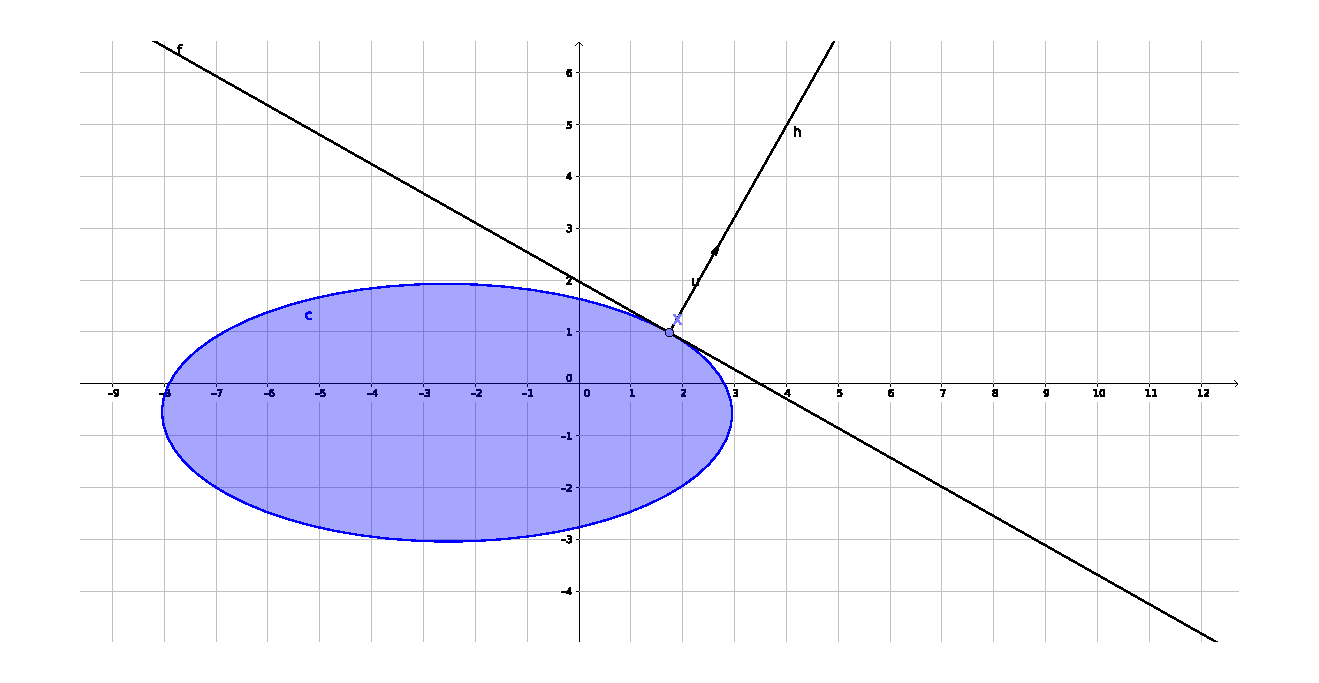
\includegraphics[width=\textwidth]{image2.pdf}

Строим гипотезу $Y = \lt\{y' \mid y' = \theta \mathbf{x} + (1-\theta)y, \forall y \in Y, \forall \theta \leq 1  \rt\}$, что геометрически представляет из себя луч проведенный из точки $\mathbf{x}$, коллинеарный вектору нормали касательной к выпуклому множеству плоскости в точке $\mathbf{x}$

Проверяем неравенство для выпуклого замкнутого множества.

Пусть $y$ - фиксированная точка, так как $S$ - выпукло и замкнуто верно:
$$ \lt\langle{\pi_S(y) - y, x' - \pi_S(y)}\rt\rangle = \lt\langle{\mathbf{x} - y, x' - \mathbf{x}}\rt\rangle \ge 0,  \forall x' \in S$$

Проверим, что это также верно и для $y' = \theta \mathbf{x} + (1-\theta)y$
 
$$\lt\langle{\mathbf{x} - \theta \mathbf{x} - (1 - \theta)y, x' - \mathbf{x}}\rt\rangle = (1-\theta)\lt\langle{\mathbf{x} - y, x' - \mathbf{x} }\rt\rangle \ge 0 \textbf{, т. к. }\theta \le 1$$
 
\vspace{\baselineskip}

Заметим, что выражение $$\lt\{y' \mid y' = \theta \mathbf{x} + (1-\theta)y, \forall y \in Y, \forall\theta \leq 1  \rt\}$$

 можно переписать как 
 
$$\lt\{y' \mid y' = \theta \mathbf{x} + (1-\theta)(\mathbf{x} + \nabla F(\mathbf{x})), \forall \theta \leq 1  \rt\}$$

Где $\nabla F(\mathbf{x})$ - вектор нормали касательной гиперплоскости в точке $\mathbf{x}$.

F(x) = 0 - уравнение поверхности $S$

\textbf{Ответ:} $Y = \lt\{y' \mid y' = \theta \mathbf{x} + (1-\theta)y, \forall y \in Y, \theta \leq 1  \rt\}$

%6
\section{}

Пусть даны $\mathbf{x} \in \mathbb{R}^n$ и выпуклый конус $K \subseteq \mathbb{R}^n$. Пусть $Y = \mathbf{x} + K$, $\mathbf{y} \in Y$. Найти множество $X \subset \mathbb{R}^n$, такое, что $\mathbf{x} \in X, \forall \mathbf{y} \in Y: x = \pi_X(\mathbf{y})$

\vspace{\baselineskip}

\textbf{Решение:}

\vspace{\baselineskip}

1. Заметим, что задача имеет тривиальное решение когда $X = {x}$ (состоит из одной точки).

\vspace{\baselineskip}

2. Мн-во $Y = \mathbf{x} + K$ соответствует смещенному конусу на вектор $\mathbf{x}$.

Геометрический подход к решению.

%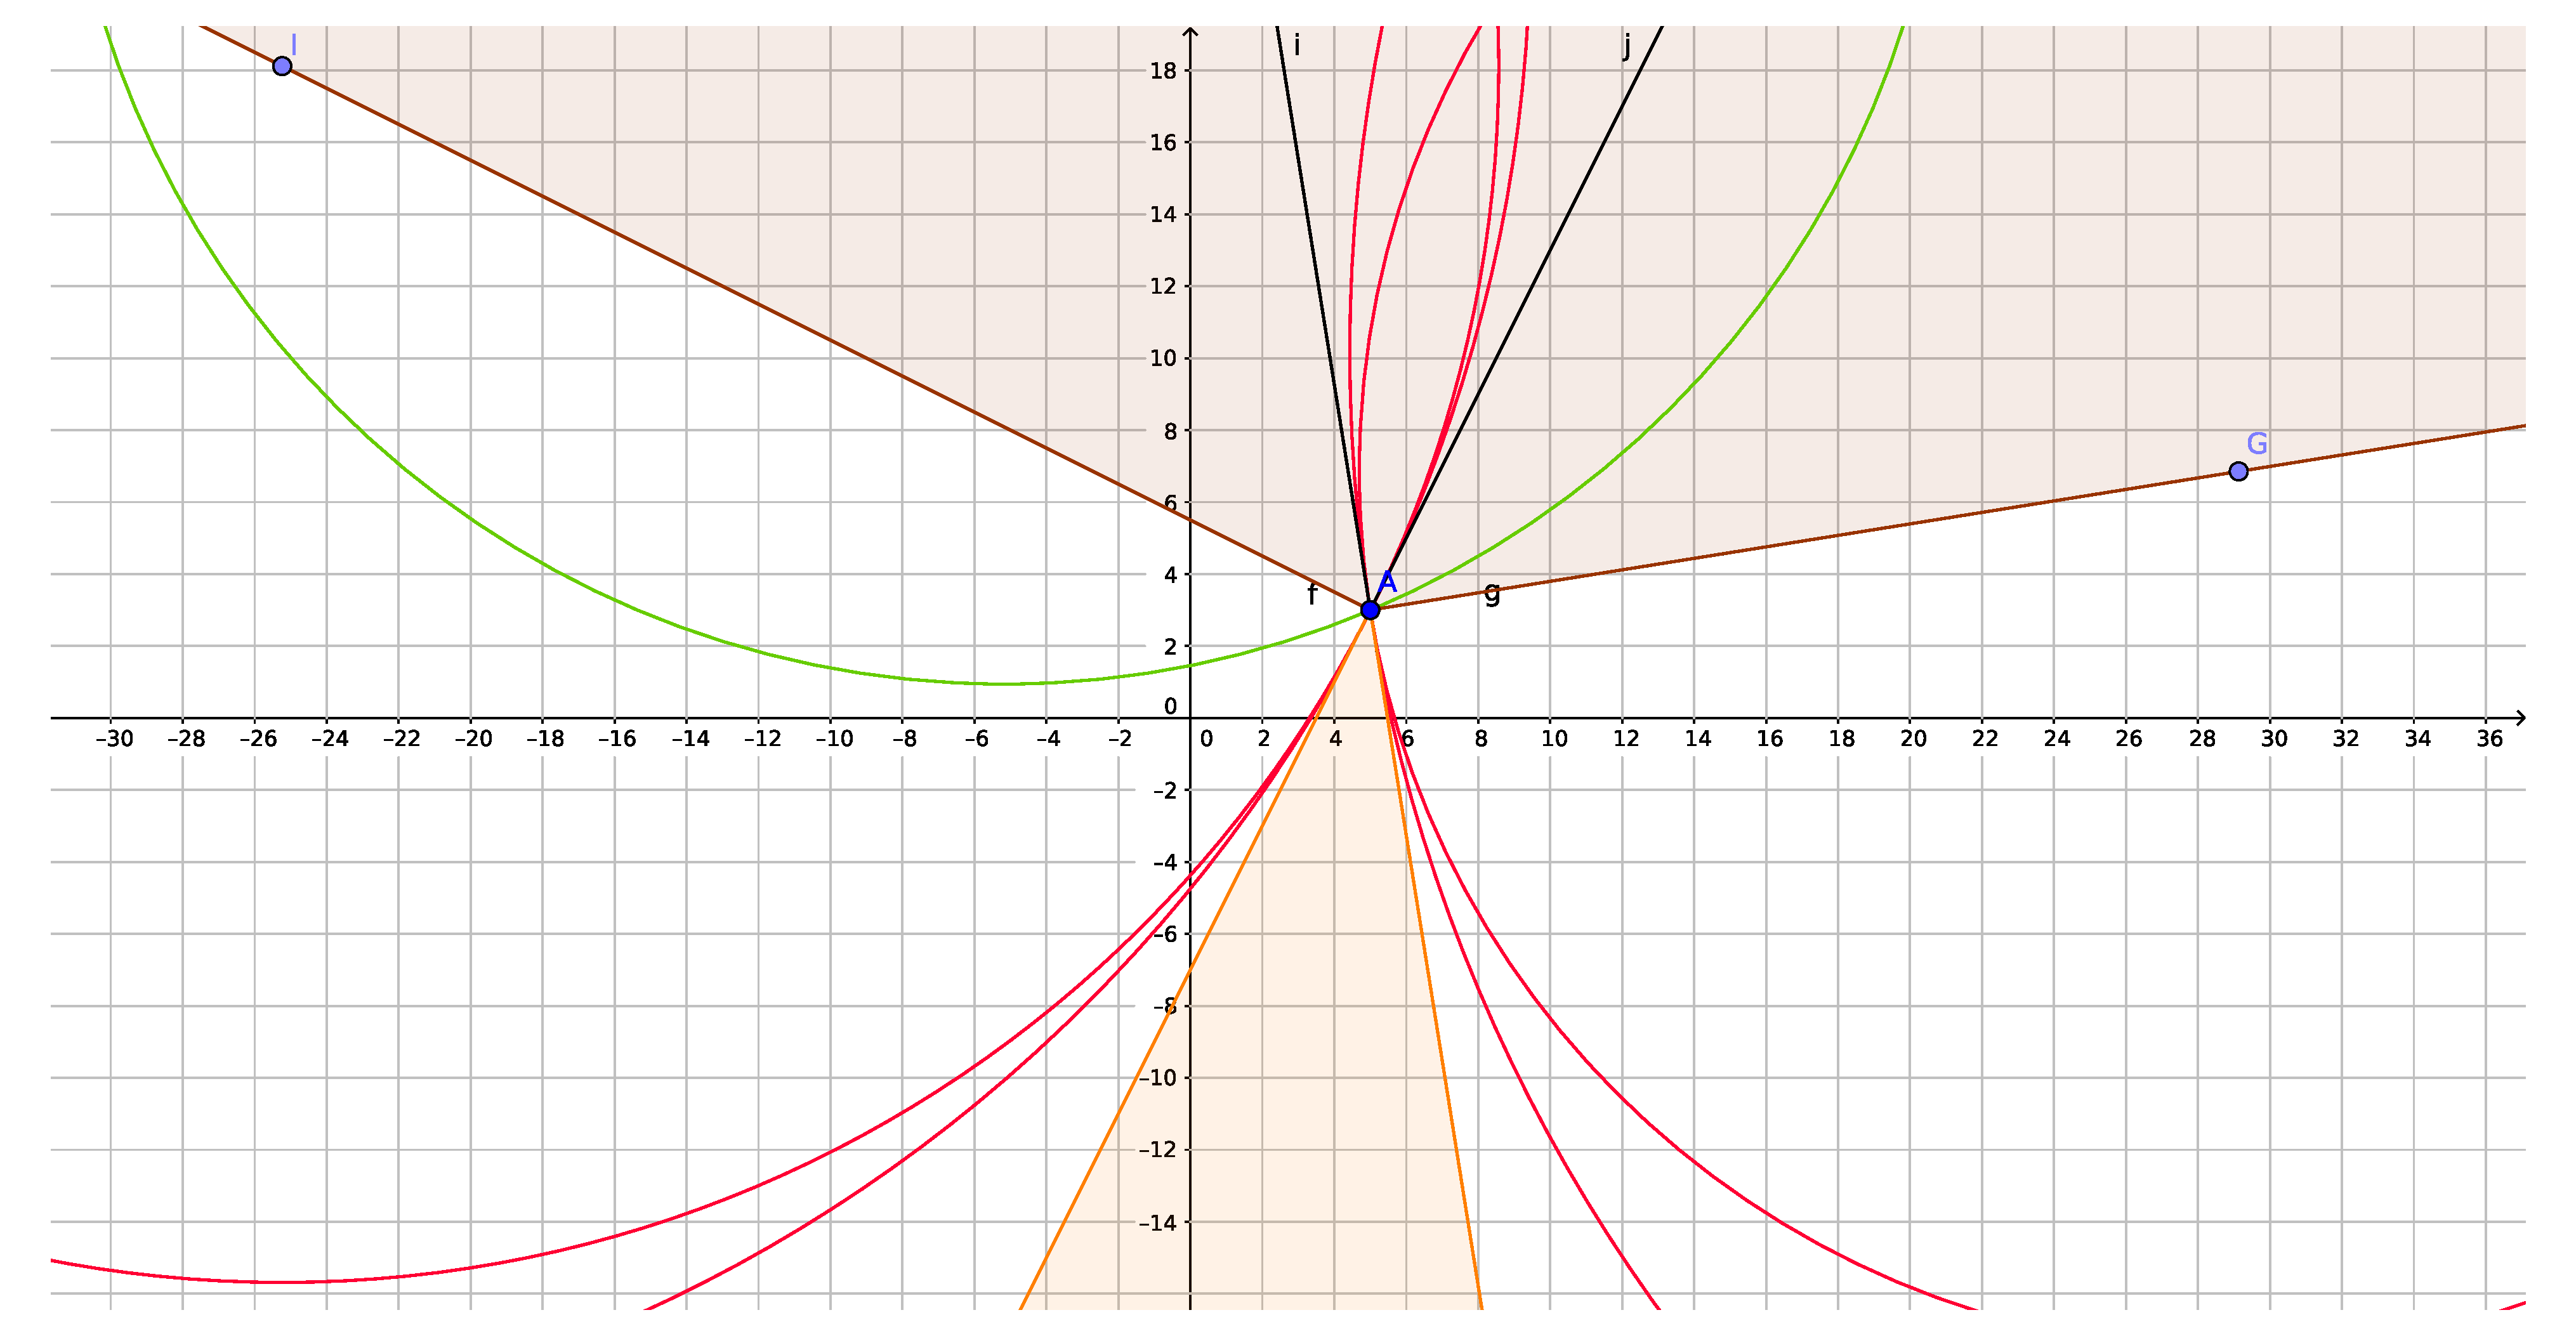
\includegraphics[width=15cm,height=7cm,keepaspectratio]{image.pdf}
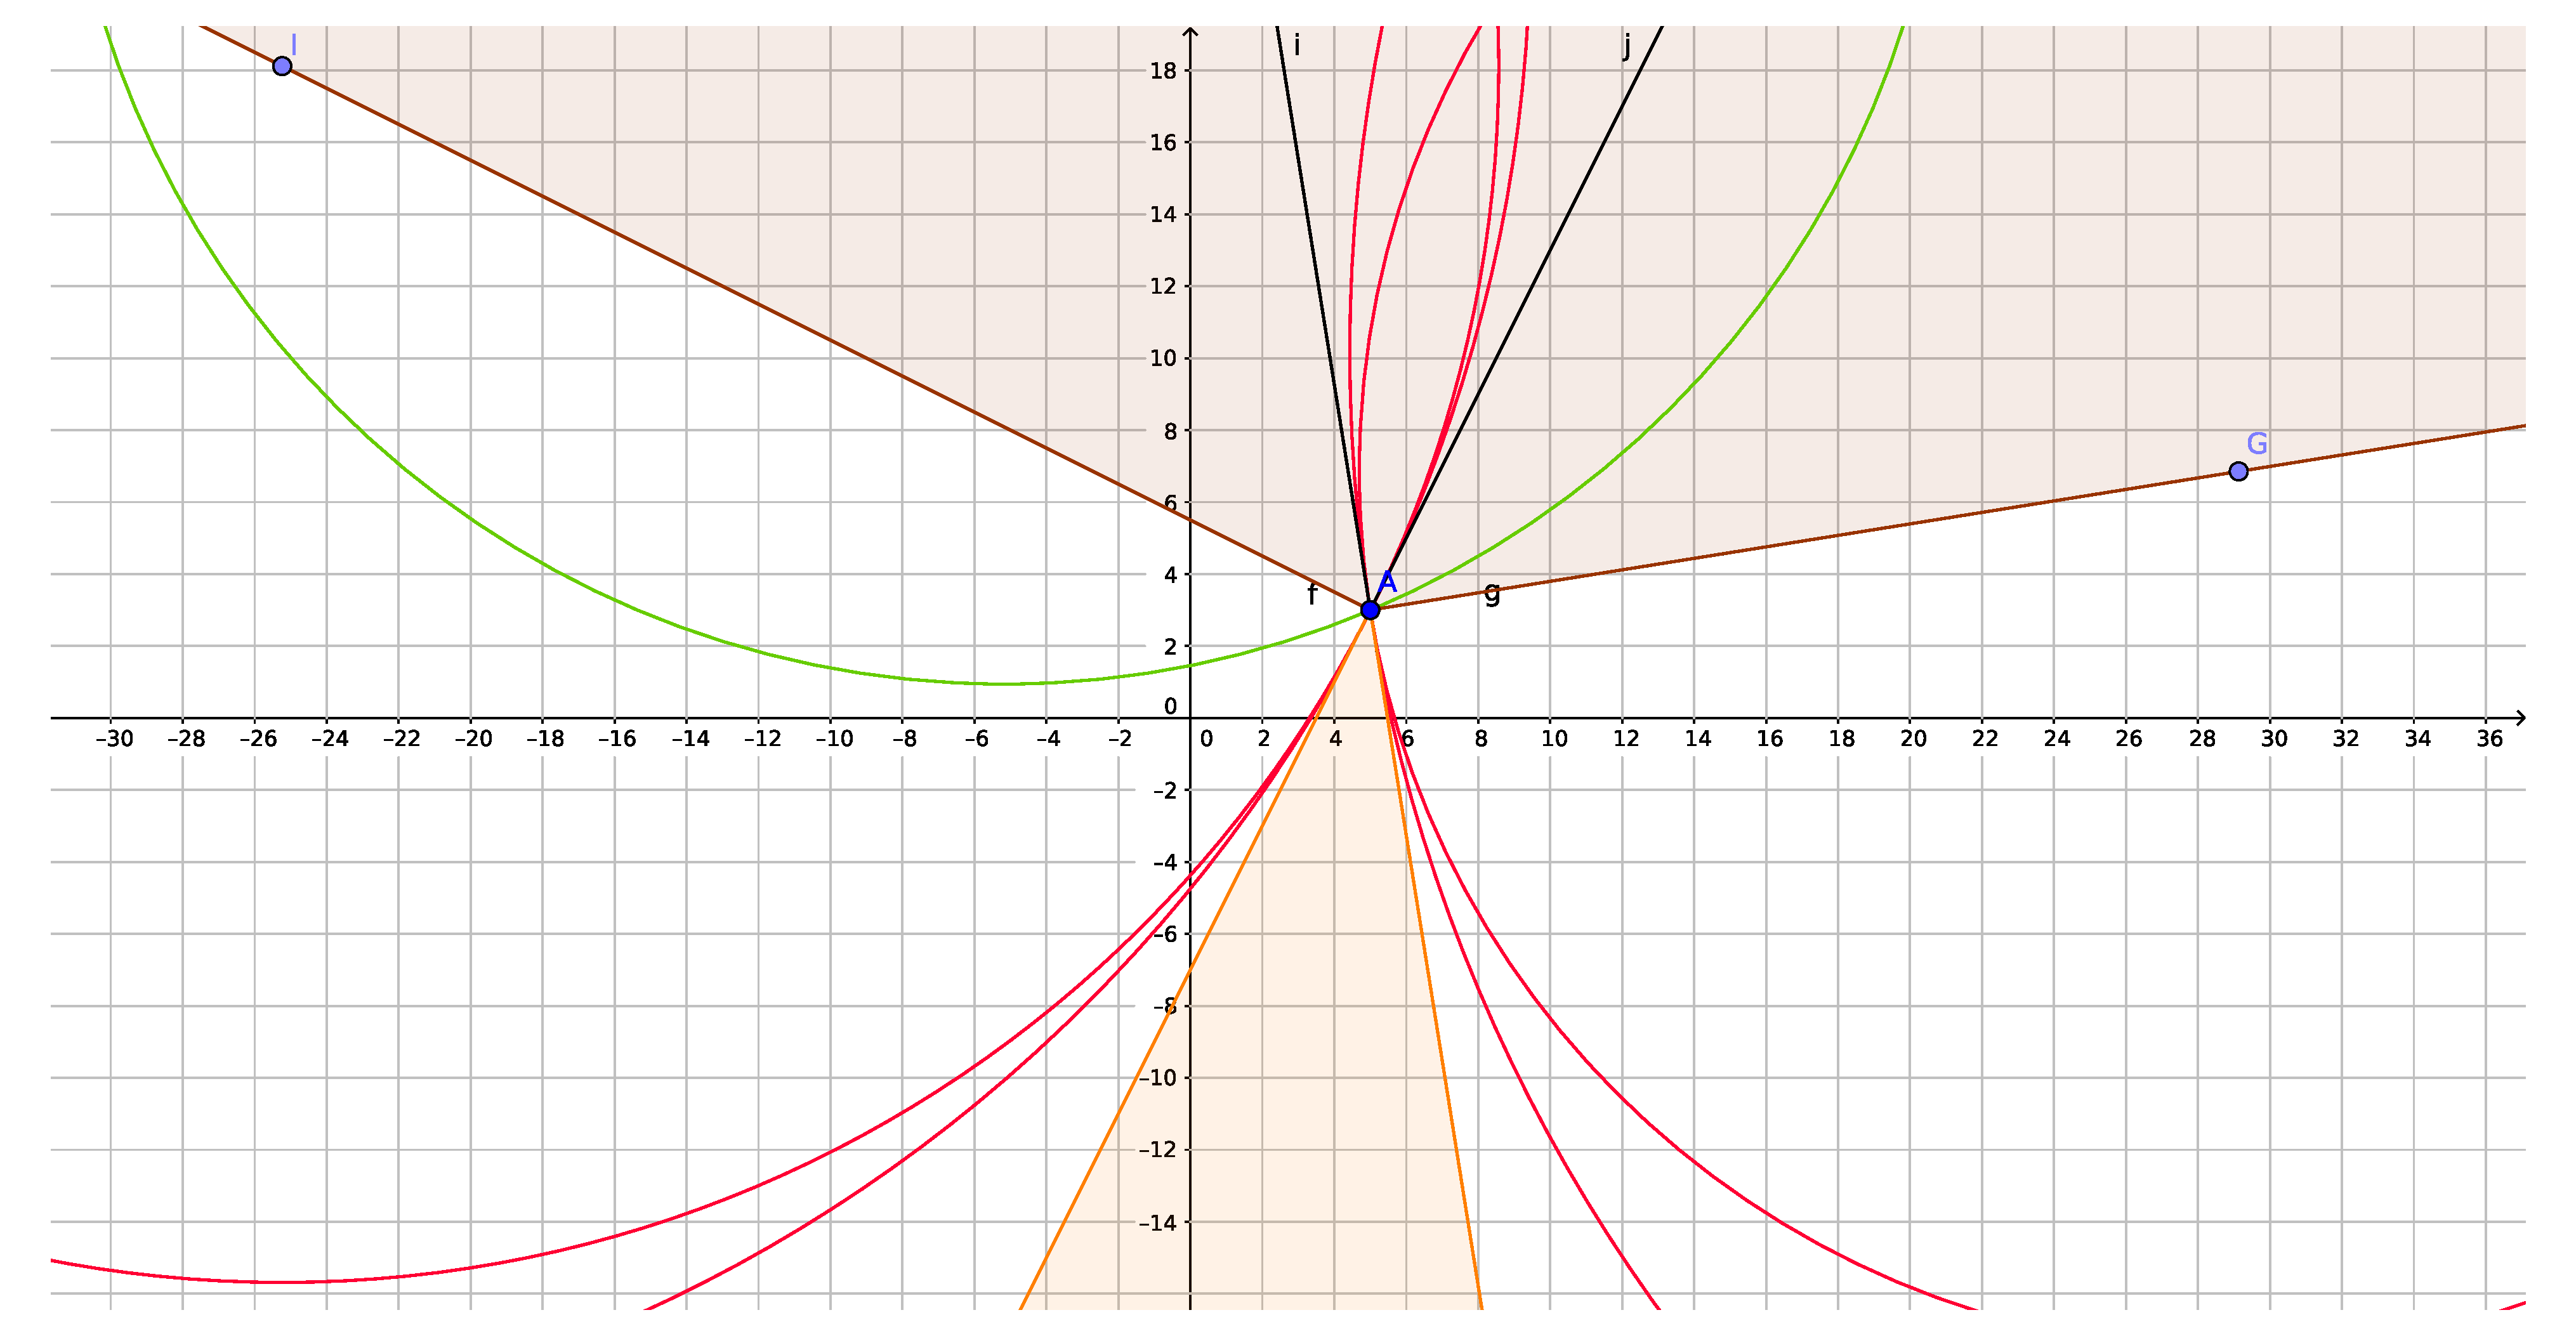
\includegraphics[width=\textwidth]{image.pdf}

\vspace{\baselineskip}

$К$ - фиолетовый конус на картинке.

Так как $\vec{0} \in K \Rightarrow \mathbf{x}$ - вершина конуса.

Рассмотрим точки на границе конуса (крайний случай) и проведем из них окружности до $\mathbf{x}$.

Так как $\forall y \in \partial Y \rightarrow \pi_X(y) = \mathbf{x}$, окружности пересекаются с $X$ только в точке $\mathbf{x}$.

Отсюда искомое множество $X$ (золотой конус на картинке) строится как касательный конус ко всевозможным окружностям с центром на $\partial Y$.

Проведенные рассуждения на $\mathbb{R}^2$ обобщаются на $\mathbb{R}^n$

\end{document} % конец документа

